% CAP description for Tree --> Expand by Textpath --> Textpath

Use this parameter to specify the textpath of the subtree you want to expand. Make sure you give the whole path (either starting from the top of the tree, or at the position defined by the pre-ascend and path type parameters). 
\begin{itemize}
\item Enter the path to the item as a textpath.
\item Use slash {\tt '/'} as a path separator (to separate parent nodes from child nodes).
\item For example, \bxshell{File/Open}  or \bxshell{Category/Horror} (without quotes). 
\item Either make sure that your path is written exactly as it appears in the interface, or use a regular expression to match the text.
\item Each segment of the path will be used to find a corresponding node, using the operator provided.
  \end{itemize}



\textbf{Example:}

\begin{itemize}
\item Your tree looks like this:

\begin{figure}
\begin{center}
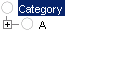
\includegraphics{PS/Treeexample3}
\caption{Tree 3}
\label{treeexample3}
\end{center}
\end{figure}

\item You want to expand the tree to node A
\item Enter \bxshell{Category/A}:

\begin{figure}
\begin{center}
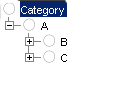
\includegraphics{PS/Treeexample4}
\caption{Tree 4}
\label{treeexample4}
\end{center}
\end{figure}
\end{itemize}
